\documentclass[a4paper,14pt]{extarticle}

% Путь до папки с общими шаблонами
\newcommand{\pathToCommonFolder}{/home/denilai/Documents/repos/latex/Common}
% Название работы в титуле
\newcommand{\workname}{Отчет по практическим работам}
% Название дисциплины в титуле
\newcommand{\discipline}{Технологические основы Инетернета вещей}
% Название кафедры в титуле
\newcommand{\kafedra}{Кафедра Математического обеспечения и стандартизации информационных технологий}
% Тема работы в титуле
\newcommand{\theme}{Знакомство с оборудованием}
% Должность преподавателя в титуле
\newcommand{\rang}{ассистент}

% ФИО студента в титуле
\newcommand{\studentfio}{К.~Ю.~Денисов}%\\Д.~Н.~Федосеев\\А.~М.~Сосунов}\\%К.~Ю.~Денисов\\%И.~А.~Кремнев
% ФИО преподавателя в титуле
\newcommand{\teacherfio}{Ю.~А.~Воронцов}


\usepackage{tabularx}


\usepackage{booktabs}
\newcolumntype{b}{X}
\newcolumntype{s}{>{\hsize=.5\hsize}X}
\newcommand{\heading}[1]{\multicolumn{1}{c}{#1}}

% установка размера шрифта для всего документа
%\fontsize{20pt}{18pt}\selectfont
\usepackage{extsizes} % Возможность сделать 14-й шрифт

% Вставка заготовки преамбулы
% Этот шаблон документа разработан в 2014 году
% Данилом Фёдоровых (danil@fedorovykh.ru) 
% для использования в курсе 
% <<Документы и презентации в \LaTeX>>, записанном НИУ ВШЭ
% для Coursera.org: http://coursera.org/course/latex .
% Исходная версия шаблона --- 
% https://www.writelatex.com/coursera/latex/5.3

% В этом документе преамбула

% Для корректного использования русских символов в формулах
% пакеты hyperref и настройки, связанные с ним, стоит загуржать
% перед загрузкой пакета mathtext



% поддержка русских букв
% кодировка шрифта
%\usepackage[T2A]{fontenc} 
\usepackage{pscyr}

% использование ненумеровонного абзаца с добавлением его в содержаниеl

\newcommand{\anonsection}[1]{\section*{#1}\addcontentsline{toc}{section}{#1}}
\newcommand{\sectionunderl}[1]{\section*{\underline{#1}}}


% настройка окружения enumerate
\usepackage{enumitem}
\setlist{noitemsep}
\setlist[enumerate]{labelsep=*, leftmargin=1.5pc}

\usepackage{hyperref}

% сначала ставить \usepackage{extsizes} % Возможность сделать 14-й шрифт
% для корректной установки полей вставлять преамбулу следует в последнюю очередь (но перед дерективой замены \rmdefault)
\usepackage[top=20mm,bottom=25mm,left=35mm,right=20mm]{geometry} % Простой способ задавать поля

\hypersetup{				% Гиперссылки
	unicode=true,           % русские буквы в раздела PDF
	pdftitle={Заголовок},   % Заголовок
	pdfauthor={Автор},      % Автор
	pdfsubject={Тема},      % Тема
	pdfcreator={Создатель}, % Создатель
	pdfproducer={Производитель}, % Производитель
	pdfkeywords={keyword1} {key2} {key3}, % Ключевые слова
	colorlinks=true,       	% false: ссылки в рамках; true: цветные ссылки
	linkcolor=red,          % внутренние ссылки
	citecolor=black,        % на библиографию
	filecolor=magenta,      % на файлы
	urlcolor=blue           % на URL
}

%%% Работа с русским языком
\usepackage{cmap}					% поиск в PDF
\usepackage{mathtext} 				% русские буквы в формулах
\usepackage[T2A]{fontenc}			% кодировка
\usepackage[utf8]{inputenc}			% кодировка исходного текста
\usepackage[english,russian]{babel}	% локализация и переносы
\usepackage{indentfirst}
\frenchspacing

%для изменения названия списка иллюстраций
\usepackage{tocloft}


\renewcommand{\epsilon}{\ensuremath{\varepsilon}}
\renewcommand{\phi}{\ensuremath{\varphi}}
\renewcommand{\kappa}{\ensuremath{\varkappa}}
\renewcommand{\le}{\ensuremath{\leqslant}}
\renewcommand{\leq}{\ensuremath{\leqslant}}
\renewcommand{\ge}{\ensuremath{\geqslant}}
\renewcommand{\geq}{\ensuremath{\geqslant}}
\renewcommand{\emptyset}{\varnothing}

% Изменения параметров списка иллюстраций
\renewcommand{\cftfigfont}{Рисунок } % добавляем везде "Рисунок" перед номером
\addto\captionsrussian{\renewcommand\listfigurename{Список иллюстративного материала}}

\newcommand{\tm}{\texttrademark\ }
\newcommand{\reg}{\textregistered\ }


%%% Дополнительная работа с математикой
\usepackage{amsmath,amsfonts,amssymb,amsthm,mathtools} % AMS
\usepackage{icomma} % "Умная" запятая: $0,2$ --- число, $0, 2$ --- перечисление

%% Номера формул
%\mathtoolsset{showonlyrefs=true} % Показывать номера только у тех формул, на которые есть \eqref{} в тексте.
%\usepackage{leqno} % Нумереация формул слева

%% Свои команды
\DeclareMathOperator{\sgn}{\mathop{sgn}}

%% Перенос знаков в формулах (по Львовскому)
\newcommand*{\hm}[1]{#1\nobreak\discretionary{}
{\hbox{$\mathsurround=0pt #1$}}{}}


% отступ для первого абзаца главы или параграфа
%\usepackage{indentfirst}

%%% Работа с картинками
\usepackage{graphicx}  % Для вставки рисунков
\graphicspath{{images/}{screnshots/}}  % папки с картинками
\DeclareGraphicsExtensions{.pdf,.png,.jpg}
\setlength\fboxsep{3pt} % Отступ рамки \fbox{} от рисунка
\setlength\fboxrule{1pt} % Толщина линий рамки \fbox{}
\usepackage{wrapfig} % Обтекание рисунков текстом

%%% Работа с таблицами
\usepackage{array,tabularx,tabulary,booktabs} % Дополнительная работа с таблицами
\usepackage{longtable}  % Длинные таблицы
\usepackage{multirow} % Слияние строк в таблице

%%% Теоремы
\theoremstyle{plain} % Это стиль по умолчанию, его можно не переопределять.
\newtheorem{theorem}{Теорема}[section]
\newtheorem{proposition}[theorem]{Утверждение}

\theoremstyle{plain} % Это стиль по умолчанию, его можно не переопределять.
\newtheorem{work}{Практическая работа}[part]


 
 
\theoremstyle{definition} % "Определение"
\newtheorem{corollary}{Следствие}[theorem]
\newtheorem{problem}{Задача}[section]
 
\theoremstyle{remark} % "Примечание"
\newtheorem*{nonum}{Решение}



%%% Программирование
\usepackage{etoolbox} % логические операторы

%%% Страница

%	\usepackage{fancyhdr} % Колонтитулы
% 	\pagestyle{fancy}
%   \renewcommand{\headrulewidth}{0pt}  % Толщина линейки, отчеркивающей верхний колонтитул
% 	\lfoot{Нижний левый}
% 	\rfoot{Нижний правый}
% 	\rhead{Верхний правый}
% 	\chead{Верхний в центре}
% 	\lhead{Верхний левый}
%	\cfoot{Нижний в центре} % По умолчанию здесь номер страницы

\usepackage{setspace} % Интерлиньяж
\onehalfspacing % Интерлиньяж 1.5
%\doublespacing % Интерлиньяж 2
%\singlespacing % Интерлиньяж 1

\usepackage{lastpage} % Узнать, сколько всего страниц в документе.

\usepackage{soul} % Модификаторы начертания


\usepackage[usenames,dvipsnames,svgnames,table,rgb]{xcolor}


\usepackage{csquotes} % Еще инструменты для ссылок

%\usepackage[style=authoryear,maxcitenames=2,backend=biber,sorting=nty]{biblatex}

\usepackage{multicol} % Несколько колонок

\usepackage{tikz} % Работа с графикой
\usepackage{pgfplots}
\usepackage{pgfplotstable}

% модуль для вставки рыбы
\usepackage{blindtext}

\usepackage{listings}
\usepackage{color}


% для поворота отдельной страницы. Использовать окружение \landscape
\usepackage{pdflscape} 
\usepackage{rotating} 


\definecolor{mygreen}{rgb}{0,0.6,0}
\definecolor{mygray}{rgb}{0.5,0.5,0.5}
\definecolor{mymauve}{rgb}{0.58,0,0.82}


% пример импорта файла
%\lstinputlisting{/home/denilai/repomy/conf/distributions}

\lstset{
	language=Python,
	basicstyle=\footnotesize,        % the size of the fonts that are used for the code
	numbers=left,                    % where to put the line-numbers; possible values are (none, left, right)
	numbersep=5pt,                   % how far the line-numbers are from the code
	numberstyle=\tiny\color{mygray}, % the style that is used for the line-numbers
	stepnumber=2,                    % the step between two line-numbers. If it's 1, each line will be numbered
	% Tab - 2 пробела
	tabsize=2,    
	% Автоматический перенос строк
	breaklines=true,
	frame=single,
	breakatwhitespace=true,
	title=\lstname 
}



\author{Кирилл Денисов}
\title{Лабораторная работа №1}
\date{\today}

\renewcommand{\withouttheme}{1}

%если нужна тема работы в отчете, то указать в скобках что-либо, иначе оаставить пустым
%\renewcommand{\withouttheme}{}
%если нужна дата представления отчета, то указать в скобках что-либо
%\renewcommand{\withoutsubmissiondate}{1}

% установка полуторного интервала
% \usepackage{setspace}  
% \onehalfspacing

% использовать Times New Roman
\renewcommand{\rmdefault}{ftm}


\begin{document}
	\thispagestyle{empty}
	% Вставка первого титульного листа
	% Есть две версии титульного листа - одиночный (titul) и групповой (titulAll)
	%\newcommand{\withouttheme}{} добавить эту переменную для определения, нужна ли тема
%     {} - нужна
%    {1} - не нужна

%\newcommand{\withoutsubmissiondate}{} добавить эту переменную для определения, нужен ли срок предоставления отчета
%     {} - нужен
%    {1} - не нужен

\renewcommand{\studentfio}{К.~Ю.~Денисов\\
			%	& & \hfill И.~А.~Кремнев \\
				& & \hfill А.~М.~Сосунов\\
				& & \hfill Д.~Н.~Федосеев}

\begin{center}
	\begin{figure}[h!]
		\begin{center}
			%\vspace{10ex}
			
\includegraphics[width=0.17\linewidth]{\pathToCommonFolder/gerb}
			%\caption{}\label{pic:first}
			%	\vspace{5ex}
		\end{center}	
	\end{figure}
	\small	МИНОБРНАУКИ РОССИИ \\
	Федеральное государственное бюджетное образовательное учреждение\\
	высшего образования\\
	\normalsize					
	\textbf{«МИРЭА – Российский технологический университет»\\
		РТУ МИРЭА}\\
	\noindent\rule{1\linewidth}{1pt}\\
	Институт информационных технологий\\ %\vspace{2ex}
	\kafedra\\
	\vspace{3ex}
	\large \textbf{\workname}  \\
	%\vspace{1ex}
	по дисциплине\\ «\discipline» \\
	\vspace{3ex}
	\if \withouttheme
	\textbf{Тема работы:}\\ <<\theme>>
	\fi
	\vspace{6ex}
	\small
	\begin{table}[h!]
		\begin{tabular}{lp{0.6\linewidth}l}
			\textbf{Выполнили:} & студенты группы ИВБО-02-19 & \\ 
			& & \hfill \studentfio \\%Д.~Н.~Федосеев\\%А.~М.~Сосунов\\%К.~Ю.~Денисов\\%И.~А.~Кремнев
			\textbf{Принял:} & \rang & \\
			& & \hfill \teacherfio\\
		\end{tabular}
	\end{table}

	\normalsize
	
	\vfill
	Москва 2021
	
\end{center}
	\newpage
	\tableofcontents
	\newpage
	%\listoftables
	

\section{Практическая работа №1.\\Знакомство с оборудованием}

\subsection {Устройство стенда}
Работа на практических занятиях проводится с использованием стенда (чемодана\textbf{ WBdemo-kit v.2}), содержащего типовой набор оборудования в <<умном доме>>.

Стенд состоит из компонентов, расположение которых можно увидеть на Рис. \ref{fig:wb-demo-kit1}-\ref{fig:wb-demo-kit2}. В таблице \ref{tab:device-list} приводится их полный список.
 
% TODO: \usepackage{graphicx} required
\begin{figure}[htpb]
	\centering
	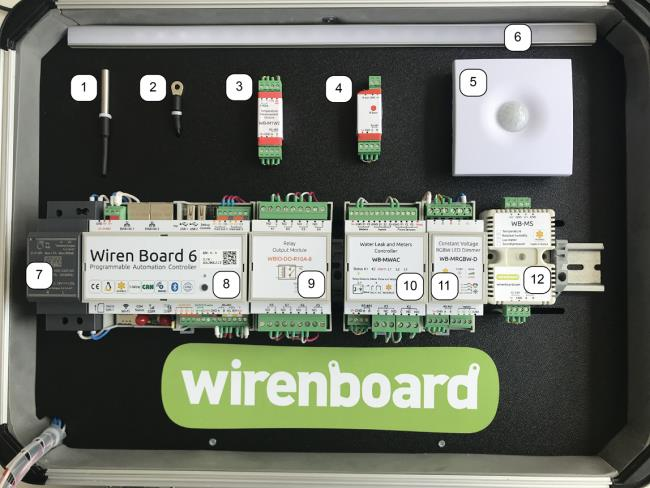
\includegraphics[width=0.6\linewidth]{images/wb-demo-kit1}
	\caption{Компоненты, расположенные на верхней крышке WB-demo-kit}
	\label{fig:wb-demo-kit1}
\end{figure}
 
 % TODO: \usepackage{graphicx} required
 \begin{figure}[htpb]
 	\centering
 	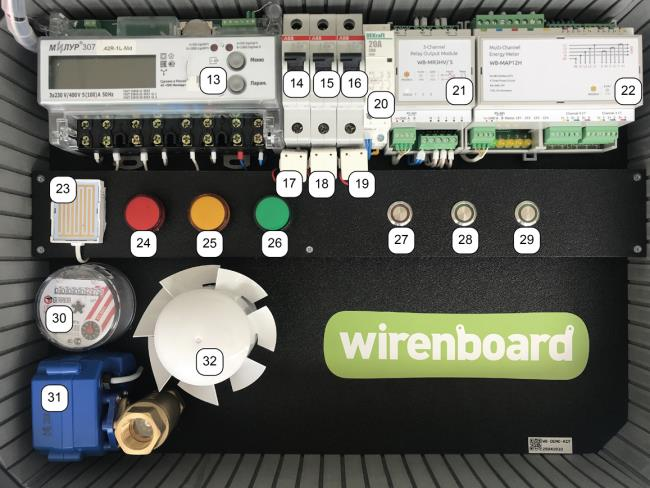
\includegraphics[width=0.6\linewidth]{images/wb-demo-kit2}
 	\caption{Компоненты, расположенные на нижней крышке WB-demo-kit}
 	\label{fig:wb-demo-kit2}
 \end{figure}

\begin{center}
	\begin{table}[htbp]
	%\small
	\begin{tabular}{|r|p{0.8\linewidth}|}
		\hline
		\multicolumn{1}{|c|}{\textbf{Номер}} & \multicolumn{1}{c|}{\textbf{Название}} \\ \hline\hline
		1 & Датчик температуры 1-wire DS18B20 \\ \hline
		2 & Датчик температуры 1-wire DS18B20 \\ \hline
		3 & Преобразователь 1-Wire — Modbus RTU WB-M1W2 \\ \hline
		4 & Устройство ИК-управления WB-MIR \\ \hline
		5 & Настенный комбинированный датчик WB-MSW v.3 \\ \hline
		6 & RGB лента в профиле \\ \hline
		7 & Блок питания HDR-30-24 \\ \hline
		8 & Контроллер Wiren Board 6 с модулем резервного питания для Wiren Board 6 WBMZ2-BATTERY \\ \hline
		9 & Модуль ввода-вывода WBIO-DO-R10A-8 \\ \hline
		10 & Модуль обнаружения протечек WB-MWAC \\ \hline
		11 & Диммер светодиодных лент на DIN-рейку WB-MRGBW-D \\ \hline
		12 & Комбинированный датчик WB-MS \\ \hline
		13 & Электросчетчик "Милур 307" \\ \hline
		14 & Автомат питания набора (L1) \\ \hline
		15 & Автомат питания вентилятора (L2) \\ \hline
		16 & Автомат питания контактора (L3) \\ \hline
		17 & Трансформатор тока 25 А (L1) \\ \hline
		18 & Трансформатор тока 25 А (L2) \\ \hline
		19 & Трансформатор тока 25 А (L3) \\ \hline
		20 & Контактор 220 В \\ \hline
		21 & Модуль реле 3-канальный WB-MR3 \\ \hline
		22 & Многоканальный измеритель WB-MAP12H \\ \hline
		23 & Датчик протечки \\ \hline
		24 & Индикатор 1 (протечка) \\ \hline
		25 & Индикатор 2 (вентилятор) \\ \hline
		26 & Индикатор 3 (контактор) \\ \hline
		27 & Кнопка 1 (подача воды, сброс аварии по протечке) \\ \hline
		28 & Кнопка 2 (вентилятор) \\ \hline
		29 & Кнопка 3 (контактор) \\ \hline
		30 & Импульсный счетчик расхода воды с имитацией потока \\ \hline
		31 & Шаровой кран с электроприводом \\ \hline
		32 & Вентилятор \\ \hline
	\end{tabular}
    \caption{Список компонентов демонстрационного набора WB-demo-kit}
	\label{tab:device-list}
\end{table}
\end{center}

	
\subsection{Ход работы}
В ходе выполнения данной практической работы были изучены и отработаны на практике следующие категории преднастроенного функционала (сценарии) стенда \textbf{Wb-demo-kit v.2}:
\begin{enumerate}
	\item Энергопотребление и контроль питания;
	\item Управление внешними силовыми устройствами;
	\item Мониторинг качества воздуха и управление вентиляцией;
	\item Мониторинг водоснабжения и протечек.
\end{enumerate}
Опишем порядок действий, производимых в рамках отработки предложенных сценариев:
\paragraph*{Включение стенда}
Убедившись, что стенд подключен к электросети, включим автоматы в порядке слева-направо, т.е. 14, 15, 16.
Включим контроллер (8), нажав на кнопку на корпусе. Когда индикатор контроллера
начнет мигать зеленым светом, контроллер будет готов к работе.
\paragraph*{Работа с функционалом контроля электропитания}
%\begin{enumerate}
	\script \textbf{Проверка наличия сетевого напряжения}
	
	Выключим автомат (14). Через несколько секунд индикатор контроллера (8) несколько раз
	часто моргнет красным и раздастся предупреждающий звуковой сигнал. Это означает, что
	сетевое напряжение отсутствует. Часть модулей продолжит питаться от встроенного в
	контроллер аккумуляторного модуля. Синий индикатор на блоке питания (7) погаснет
	примерно через 30 секунд.
	
	% TODO: \usepackage{graphicx} required
	\begin{figure}[htbp]
		\centering
		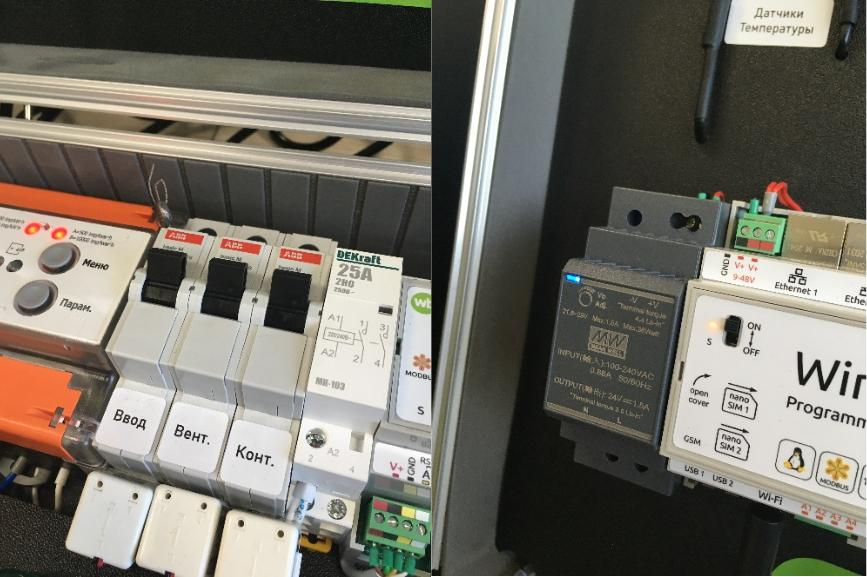
\includegraphics[width=0.6\linewidth]{images/1}
		\caption{Наличие сетевого напряжения}
		\label{fig:1}
	\end{figure}
	\script \textbf{Контроль повышенного энергопотребления}
	
	Включим вентилятор кнопкой (28). Загорится зеленая подсветка кнопки. Через некоторое
	время загорится желтый индикатор (25) --- это означает, что счетчик (22) детектирует
	энергопотребление на фазе, к которой подключен вентилятор. Не касаясь лопастей
	вентилятора, остановим его. Через несколько секунд счетчик (22) определит повышенное
	энергопотребление застопоренного вентилятора и контроллер отключит его. Погаснет
	зеленая подсветка кнопки (28), а затем -- желтый индикатор (25).	

% TODO: \usepackage{graphicx} required
\begin{figure}[htbp]
	\centering
	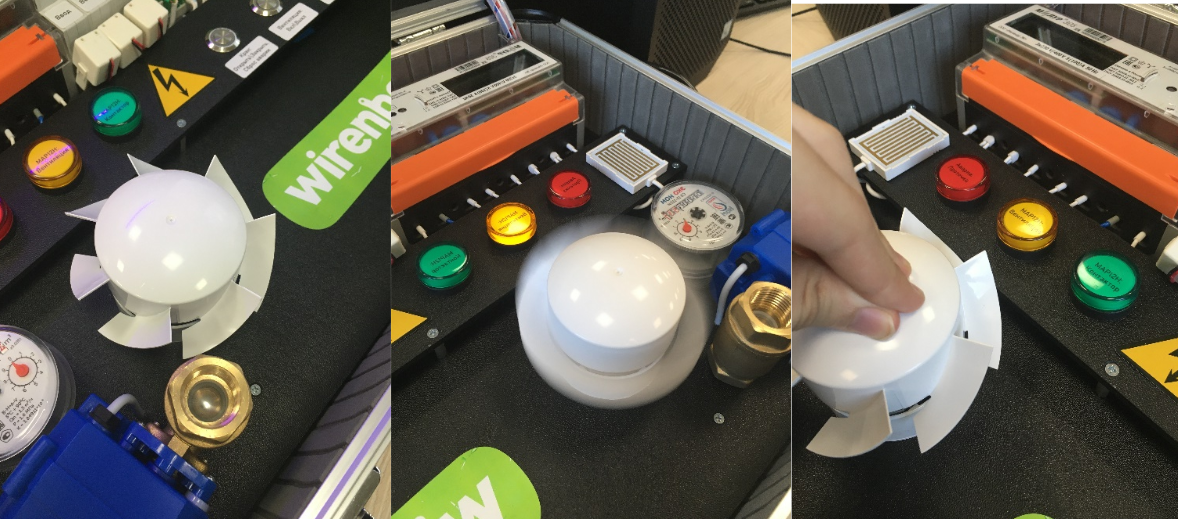
\includegraphics[width=0.6\linewidth]{images/fan}
	\caption{Контроль повышенного энергопотребления}
	\label{fig:fan}
\end{figure}

	
	\script  \textbf{Контроль автоматов}
	
	Отключим автоматы (15) и (16). Через несколько секунд начнет мигать подсветка кнопок
	(28) и (29), что означает, что напряжение на выходах автоматов пропало. Включим
	автоматы снова -- подсветка кнопок перестанет мигать.	
	
	% TODO: \usepackage{graphicx} required
	\begin{figure}[htbp]
		\centering
		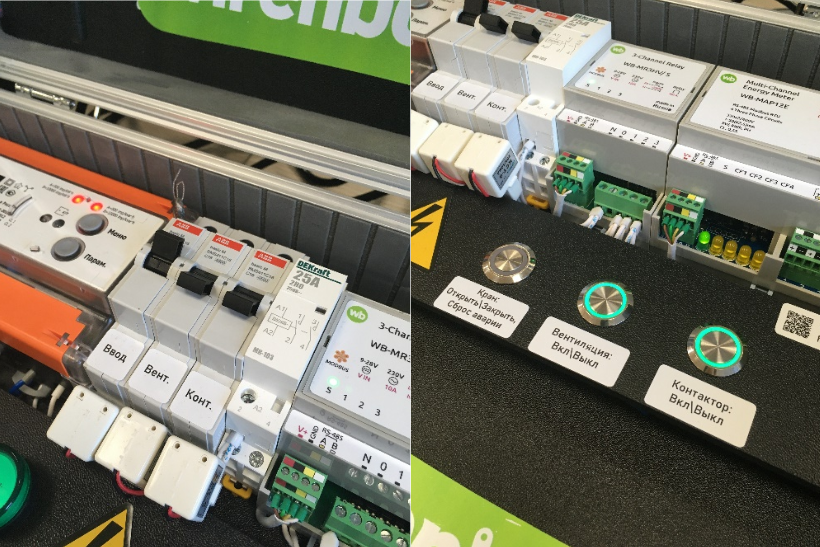
\includegraphics[width=0.6\linewidth]{images/power-off}
		\caption{Контроль автоматов}
		\label{fig:power-off}
	\end{figure}
	
%\end{enumerate}
\paragraph* {Управление внешними силовыми устройствами}
	\script \textbf{Управление контактором}

	Нажмем кнопку (29). Подсветка кнопки загорится зеленым, при этом сработает
	контактор (20). Через некоторое время загорится индикатор (26), что означает обнаружение
	энергопотребления на соответствующей фазе счетчиком (22). Нажмем кнопку (29) --
	контактор выключится, подсветка кнопки погаснет, а через несколько секунд погаснет и
	индикатор энергопотребления (26).
\paragraph*{Мониторинг качества воздуха}
	\script \textbf{Определение уровня $CO_2$} 
	
	При допустимом уровне концентрации $CO_2$ в помещении индикатор датчика (5)
	мигает зеленым светом. Если несколько раз на него энергично подуть, то через 15-20 секунд
	индикатор начнет мигать красным, что свидетельствует о превышении концентрации $CO_2$.
	При достижении нормальной концентрации датчик снова будет мигать зеленым.
\paragraph*{Мониторинг водоснабжения и протечек}
	\script \textbf{Работа модуля защиты от протечек}
	
	Нажмем кнопку (27). Откроется шаровой кран (31), а счетчик (30) начнет вращаться,
	имитируя поток воды в системе водоснабжения. Прикоснемся с небольшим усилием
	слегка влажным пальцем или смоченной салфеткой к датчику протечки.
	
	Шаровой кран перекроет поток воды, счетчик перестанет
	вращаться, загорится красный индикатор протечки (24), подсветка кнопки (27) начнет
	мигать, а модуль обнаружения протечек (10) будет выдавать непрерывный звуковой сигнал
	(на самом модуле будет гореть индикатор \textit{Alarm}). Для сброса аварийной ситуации
	(<<Протечка устранена>>) снова нажмем кнопу (27).
	Кнопкой 27 можно открывать и закрывать шаровой кран с электроприводом,
	последовательно нажимая на нее.
	
	% TODO: \usepackage{graphicx} required
	\begin{figure}[htbp]
		\centering
		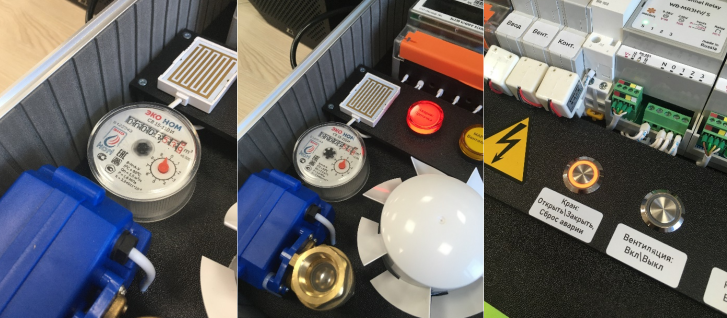
\includegraphics[width=0.6\linewidth]{images/waterproof}
		\caption{Мониторинг водоснабжения и протечек}
		\label{fig:waterproof}
	\end{figure}
	
\paragraph*{Выключение стенда}
	Для выключения оборудования сначала выключим контроллер (8), после -- автоматы в
	порядке справа-налево (т.е. 16, 15, 14).
	
\anonsubsection{Вывод}
В ходе данной практической работы мы познакомились с демонстрационным стендом\textbf{ WB-demo-kit v.2}, изучили и отработали на практике основные сценарии взаимодействия с входящими в его состав компонентами.
\newpage
\section{Практическая работа №2.\\Настройка удаленного подключения}
\subsection{Ход работы}
Задание:
\begin{enumerate}
	\item Включите стенд 
    \item Подключитесь к стенду через веб интерфейс 
	\item Запустите преднастроенные сценарии еще раз, отследить изменение параметров в веб-интерфейсе 
	\item Зафиксируйте изменения параметров в веб-интерфейсе, возникшие при выполнении сценариев
	\item Выключите стенд
\end{enumerate}


\paragraph {Выбираем уровень доступа:}
Укажем уровень доступа в веб-форме.
% TODO: \usepackage{graphicx} required
\begin{figure}[hbpt]
	\centering
	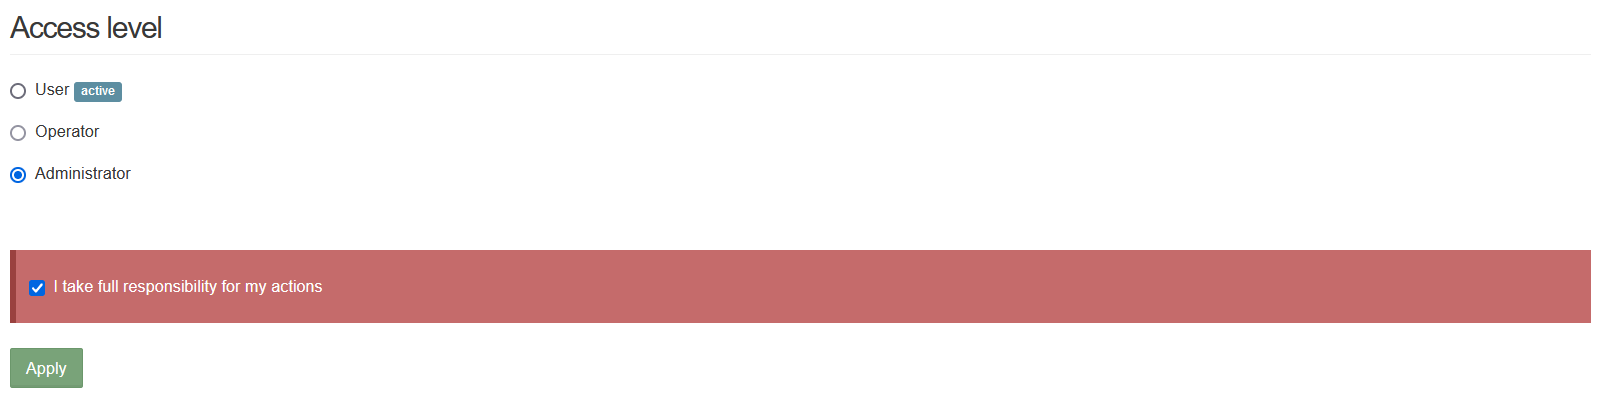
\includegraphics[width=0.6\linewidth]{images/access}
	\caption{Уровень доступа}
	\label{fig:access}
\end{figure}

\paragraph {Наличие сетевого напряжения}
Отключаем напряжение, проверяем показания датчиков энергопотребления:

% TODO: \usepackage{graphicx} required
\begin{figure}[hbpt]
	\centering
	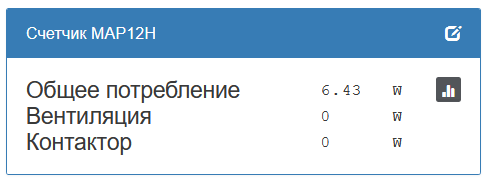
\includegraphics[width=0.5\linewidth]{images/net1}
	\caption{Наличие сетевого напряжения}
	\label{fig:net1}
\end{figure}
\newpage
% TODO: \usepackage{graphicx} required
\begin{figure}[hbpt]
	\centering
	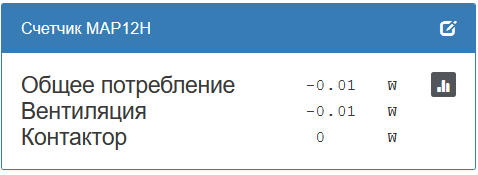
\includegraphics[width=0.5\linewidth]{images/net2}
	\caption{Изменение сетевого напряжения}
	\label{fig:net2}
\end{figure}

\ref{fig:fan-gui}
\paragraph{Контроль повышенного энергопотребления}
Включили вентилятор, прижали рукой, загорелся индикатор и сработала сигнализация, вентилятор выключился:
% TODO: \usepackage{graphicx} required
\begin{figure}[hbpt]
	\centering
	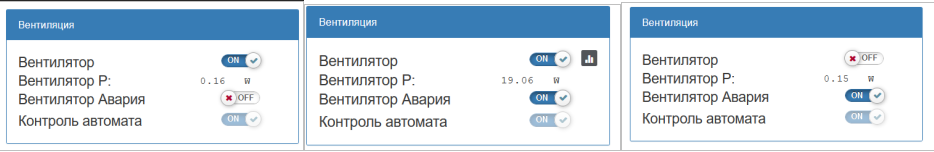
\includegraphics[width=0.6\linewidth]{images/fan-gui}
	\caption{Контроль повышенного энергопотребления}
	\label{fig:fan-gui}
\end{figure}

\paragraph{Контроль автоматов}
Отключаем питание, загораются указанные кнопки:

% TODO: \usepackage{graphicx} required
\begin{figure}[hbpt]
	\centering
	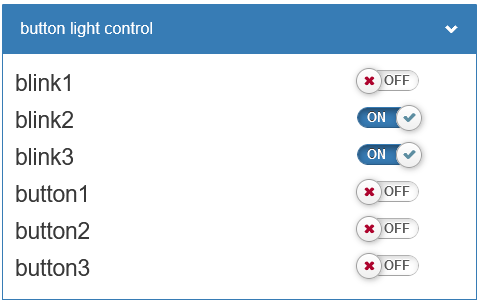
\includegraphics[width=0.5\linewidth]{images/auto-gui}
	\caption{Контроль автоматов}
	\label{fig:auto-gui}
\end{figure}
\paragraph{Контроль повышенного энергопотребления}
Включили вентилятор, прижали рукой, загорелся индикатор и сработала сигнализация, вентилятор выключился

\anonsubsection{Вывод}
В ходе данной практической работы мы выполнили настройку удаленного подключения к демонстрационному стенду  WB-demo-kit, ознакомились с веб-интерфейсом, научились снимать данные с датчиков с его помощью.

\newpage
\section{Практическая работа №3. \\Обработка событий в системах\\Интернета вещей}

\subsection{Ход работы}

\paragraph {Задание:}

Разработайте сценарии для обработки событий согласно вариантам и приведите в отчете его листинг с комментариями.

Вариант №5:
\begin{enumerate}
	\item Включение и выключение вентилятора по датчику движения.
	
	\item Включение и выключения индикации зеленым и красным светом комбинированного датчика 5 по кнопкам.
\end{enumerate}
\paragraph{Разработанные скрипты} Приведем содержание разработанных скриптов на языке JavaScript:
\setcounter{script}{0}
\script Включение и выключение вентилятора по датчику движения.
\lstinputlisting{/home/denilai/Documents/repos/latex/scripts/iot-script-1.js}
\newpage
Результат выполнения сценария:
% TODO: \usepackage{graphicx} required
\begin{figure}[htbp]
	\centering
	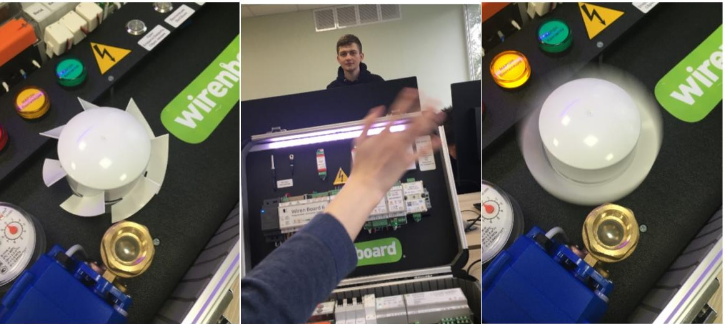
\includegraphics[width=0.7\linewidth]{images/script1-result}
	\caption{Результат 1}
	\label{fig:script1-result}
\end{figure}


\script Включение и выключения индикации зеленым и красным светом комбинированного датчика 5 по кнопка
\lstinputlisting{/home/denilai/Documents/repos/latex/scripts/iot-script-2.js}
\anonsubsection{Вывод}
В ходе данной практической работы мы получили начальные навыки написания скриптов (сценариев) для стенда WB-demo-kit  на языке JavaScript, познакомились с понятием <<правил>>, написали собственные сценарии и проверили их работоспособность на практике. 

\newpage

\section{Практическая работа №4. \\Основы электротехники в системах\\Интернета вещей}
\subsection{Ход работы}
\paragraph{Описание сценариев} Приведем sequence диаграмму, построенные на основании первого сценария, описанного выше.
% TODO: \usepackage{graphicx} required
\begin{figure}[htbp]
	\centering
	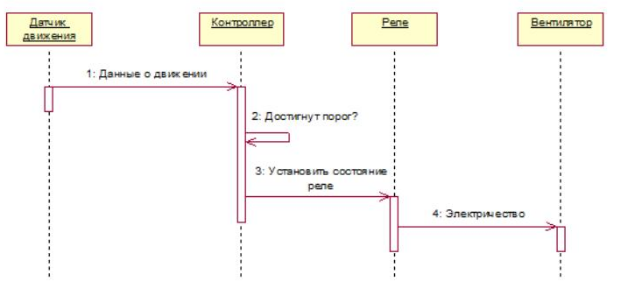
\includegraphics[width=0.7\linewidth]{images/deploy-scheme}
	\caption{Sequence диаграмма по первому сценарию}
	\label{fig:deploy-scheme}
\end{figure}

Приведем схему подключения элементов, необходимых для реализации первого сценария.
% TODO: \usepackage{graphicx} required
\begin{figure}[htbp]
	\centering
	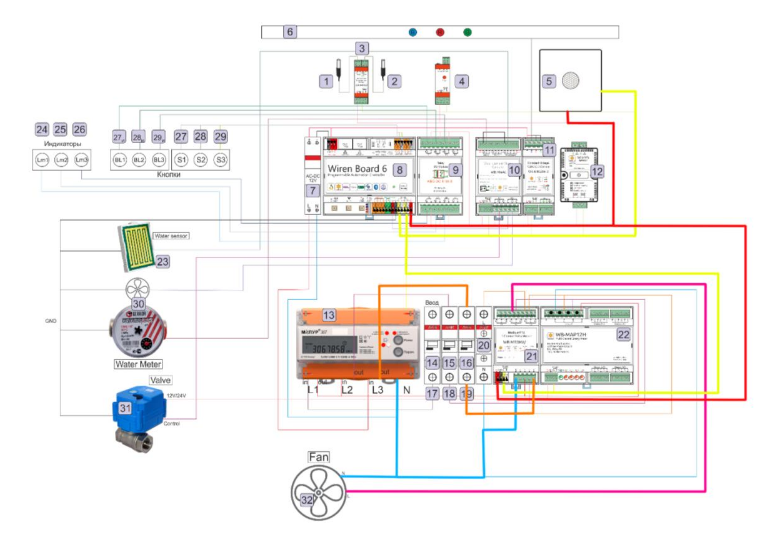
\includegraphics[width=0.7\linewidth]{images/deploy-scheme-demo}
	\caption{Схема подключения по первому сценарию}
	\label{fig:deploy-scheme-demo}
\end{figure}
Приведем sequence диаграмму, построенные на основании второго сценария, описанного выше.
% TODO: \usepackage{graphicx} required
\begin{figure}[htbp]
	\centering
	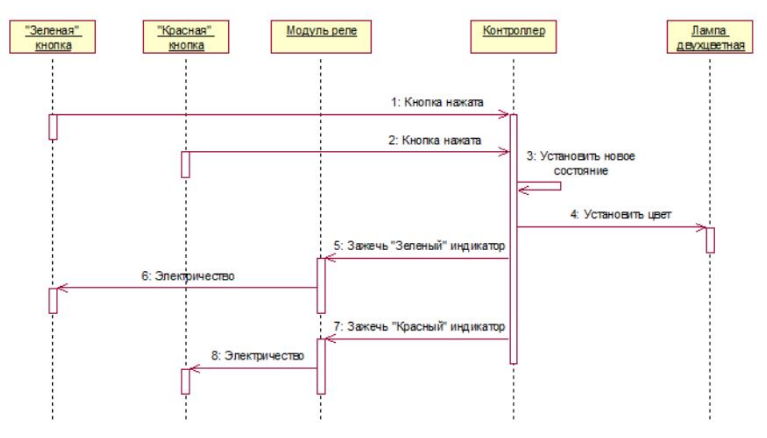
\includegraphics[width=0.7\linewidth]{images/deploy-scheme2}
	\caption{Sequence диаграмма по второму сценарию}
	\label{fig:deploy-scheme2}
\end{figure}
Приведем схему подключения элементов, необходимых для реализации второго сценария.
% TODO: \usepackage{graphicx} required
\begin{figure}[htbp]
	\centering
	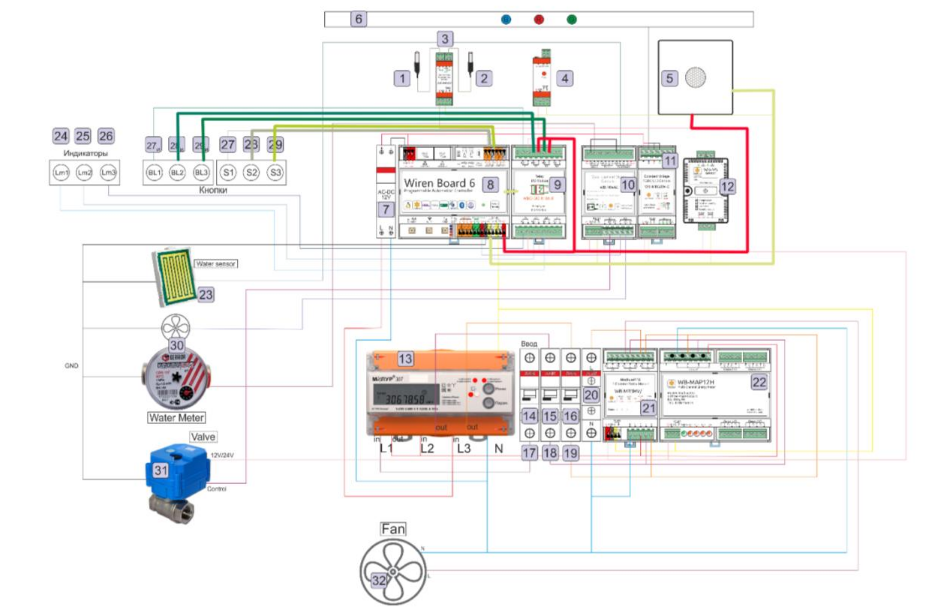
\includegraphics[width=0.7\linewidth]{images/deploy-scheme-demo2}
	\caption{Схема подключения по второму сценарию}
	\label{fig:deploy-scheme-demo2}
\end{figure}
\anonsubsection{Вывод}
В ходе данной практической работы мы описали созданные сценарии в методологии UML с помощью sequence диаграмм, продумали схему подключения модулей и компонентов, необходимых для их реализации.





\end{document}


